% En LaTeXfil slutter med .tex
% Kommentarer begynner med %.

% Delen før \begin{document} heter "preamble". Her setter du innstillinger som
% gjelder for hele dokumentet og angir hvilke pakker du bruker.
% Pakker importeres med \usepackage{}. Hver pakke har sin egen dokumentasjon som
% du kan søke opp på https://www.ctan.org

\documentclass[a4paper, 12pt, norsk]{article}
% En side har størrelse A4, normal tekststørrelse er 12pt, språk er bokmål (se
% \usepackage{babel} under). ‘article’ er bra for de fleste korte dokumenter,
% som f.eks. oppgavebesvarelser.
% Se https://en.wikibooks.org/wiki/LaTeX/Document_Structure#Preamble for detaljer
% om innstillingene.

\usepackage[utf8]{inputenc}
% Bruk UTF8 enkoding. Du kan lese mer om tekstenkoding og hvorfor det er viktig her:
% https://www.w3.org/International/questions/qa-what-is-encoding

\usepackage[norsk]{babel}
% Bruk ‘norsk’ for å skrive bokmål, ‘nynorsk’ for å skrive nynorsk.

\usepackage[table, usenames, svgnames]{xcolor} % gjør det mulig å bruke farger.
% Liste over navngitte farger finnes i dokumentasjonen (del 4, fra side 39).

\usepackage{physics} % enklere kommandoer for å skrive bl.a. vektorer, deriverte,
% matriser og notasjon ofte brukt i fysikk.

\usepackage{siunitx} % kommandoer for SI-enheter.

\usepackage{graphicx} % for å legge til figurer.

\usepackage{listings}
% Denne pakken lar deg inkludere kode i dokumentet.

\usepackage{hyperref} % for å lage klikkbare lenker.

\usepackage{cleveref} % smartere henvisninger enn den innebygde kommandoen \ref.


% Innstillinger for teksten, hvis du vil ha noe annet enn standardinstillingene:
\setlength{\parindent}{1em} % innrykk på begynnelsen av avsnitt. 1em er bredden til M.
\setlength{\parskip}{1ex} % ekstra avstand mellom avsnitt. 1ex er høyden til x.
\linespread{1} % linjeavstand

% Endre hvordan seksjonsnummer skrives:
\renewcommand{\thesection}{\Roman{section}}
\renewcommand{\thesubsection}{\Roman{section}--\arabic{subsection}}
\renewcommand{\thesubsubsection}{\alph{subsection})}

% Instillinger for listings pakken
\lstset{
	% Ekstra tegn
	literate=  % Ekstra tegn som brukes i koden må legges til her.
		{æ}{{\ae}}1 {Æ}{{\AE}}1
		{ø}{{\o}}1 {Ø}{{\O}}1
		{å}{{\r a}}1 {Å}{{\r A}}1,
	% Utseende
	backgroundcolor=\color[rgb]{.9, .9, .9}, % Husk komma mellom hvert argument.
	basicstyle=\scriptsize\ttfamily, % mindre skrift og fast bredde font
	commentstyle=\color{SeaGreen},
	keywordstyle=\color{Blue},
	stringstyle=\color{MediumOrchid},
	showstringspaces=false, % Hvis true vises mellomrom som ␣i tekststrenger.
	numbers=left, % vis linjenummer til venstre
	numbersep=5pt, % avstand mellom linjenummer og kode
	stepnumber=5, % nummerer hver femte linje
	numberstyle=\tiny\color{Gray}, % bruk liten lysegrå skrift for linjenummer
}

\title{Introduksjon til \LaTeX} % tittel
\author{Johannes Sørby Heines} % forfatter

% Dette er slutten på preamble. Hvis du vil bruke samme preamble i flere dokumenter
% kan du lagre den i en egen min_preamble.tex fil, og så skrive \input{min_preamble.tex}
% før \begin{document}. Kommandoen \input{} gjør at LaTeX tolker innholdet i inputfilen
% som om du hadde skrevet det rett inn i hovedfilen.

\begin{document}

\maketitle  % Setter opp tittel, forfatter og dato.

\begin{abstract} % Sammendrag som dette er nødvendig for vitenskapelige rapporter og artikler.
	Dette dokumentet er laget for å gi en innføring i \LaTeX, med nok informasjon til å skrive
	det som forventes av oppgavebesvarelser og rapporter i løpet av bachelorstudiet.
	Jeg går gjennom overskrifter, henvisninger, likninger, figurer og programkode,
	samt flere nyttige pakker for skriving i fysikk og generelt.
	Jeg forsøker å gi en forståelse av prinsippene i \LaTeX som vil gjøre det lettere å lete
	seg fram til mer informasjon der det trengs.
	Forslag til forbedringer mottas med takk på \url{https://github.com/johashei/LaTeXintro}.
	Der ligger også den nyeste versjonen av dette dokumentet.
\end{abstract}


Åpne dette dokumentet i en tex-editor slik at du lett kan se både tex-filen og den
genererte pdf-en.

\section{Dette er en overskrift.}
Hvis du bruker \lstinline[language=tex, basicstyle=\ttfamily]$\documentclass[...]{report}$
har du også kapitler, som kommer før overskrifter.

\subsection{Dette er en underoverskrift.}
Teksten ser lik ut uavhengig av hvor mange overskriftnivåer du har.

\subsubsection{Dette er en underunderoverskrift.}
Hvis du trenger tre overskriftnivåer bør du tenke deg om. Blir teksten klarere
om den omstruktureres?

Som du ser over kommer det ikke innrykk på første avsnitt etter en overskrift, innrykket
kommer derimot når et avsnitt følger et annet.

\section{Nummerering}

\lstset{language=tex} % Setter listings instillinger for av vise LaTeX-kode.

\subsection{Overskrifter}

Du kan fritt endre hvordan overskrifter nummereres ved å redefinere kommandoene
\lstinline$\thesection$, \lstinline$\thesubsection$, og \lstinline$\thesubsubsection$.
Prøv deg fram og finn hva som passer best.

\subsection*{Overskrift uten nummer}
Du kan også lage en overskrift uten nummer ved å sette en * mellom kommandoen og \{\}, slik:
\lstinline$\subsection*{Overskrift uten nummer}$.
Nest overskrift vil fortsette fra den forrige nummererte overslriften, som dette:

\subsection{Henvisninger}\label{ov:henvisninger}
Det kan ofte være hensiktsmessig å vise til en bestemt seksjon i teksten. Hvis du skriver
f.eks. ``Se avsnitt II--2'', men så bestemmer deg for å flytte denne delen eller legge til
en annen del før, må du endre alle henvisninger manuelt.
For å slippe det kan du sette merker på overskrifter med kommandoen \lstinline$\label{}$
og henvise til den med \lstinline$\ref{}$ eller \lstinline$\cref{}$. Den første er
innebygd i \LaTeX og gjør ikke annet enn å gi deg nummeret: \ref{ov:henvisninger}.
Den andre ligger i pakken cleveref og vet også hva du refererer til: \cref{ov:henvisninger}.


\section{Matematikk}

En av hovedgrunnene til å bruke \LaTeX\ er å skrive matematikk. Det finner flere måter å
gjøre dette på, som passer til forskjellige formål.

Når matematikken skal være integrert i teksten -- såkalt ``inline'' -- skrives den mellom
\lstinline{\( \)}. For eksempel \(r\exp(\theta i) = r\cos(\theta) + ir\sin(\theta)\). For
uttrykk som krever litt mer plass brukes \lstinline{\[ \]} -- kalt ``display'', for eksempel
\[
	f(x) \approx \sum_{n=0}^{\infty} \frac{(x-a)^n}{n!}\dv[n]{f}{x}\qty(a) .
\]
Husk at også likninger som skrives på denne måten skal kunne leses som en del av teksten, så
sett komma eller punktum etter dem.


Ren \TeX, som \LaTeX\ er basert på, bruker \lstinline{$ $} og \lstinline{$$ $$} for henholdsvis
inline- og display-matematikk, og dette fungerer også i \LaTeX, men kommandoene over er anbefalt.

For lengre utledninger er det fint å kunne sette likninger pent under hverandre, det gjør vi
med \lstinline$align$. Her brukes \lstinline{&} for å markere referansepunktet, og \lstinline{\\}
for å markere linjeskift.

\begin{align}
	\dv{N}{t} &= -\frac{N}{\tau}  \label{eq:difflikning} \\
	\frac{1}{N}\dv{N}{t} &= -\frac{1}{\tau}  \nonumber \\
	\int \frac{1}{N} \dd{N} &= \int -\frac{1}{\tau} \dd{t} \\
	\ln(N) &= -\frac{t}{\tau}  \nonumber \\
	N &= e^{-t/\tau} \label{eq:svar}
\end{align}

Som med overskrifter kan du bruke \lstinline$\label{}$ og \lstinline$\ref{}$ eller
\lstinline$\cref{}$ for å enkelt vise til en bestemt likning.
For eksempel er \cref{eq:svar} formelen for radioaktivt henfall.
\lstinline$\nonumber$ fjerner nummereringen for én likning, hvis du vil fjerne nummerering
for alle kan du bruke \lstinline$align*$.

\section{Figurer}

Figurer i vitenskapelige tekster skal ha nummer og figurtekst under.
\LaTeX\ forsøker å plassere figurer slik at det ikke blir for mye tomrom i teksten. Det betyr
at figurer ofte ikke ender opp akkurat der du definerer dem i tex-filen. Du kan sende ekstra
instruksjoner om hvordan figuren skal plasseres:
\begin{itemize}
	\item \texttt{h}: ``here'' Finn den beste plasseringen i nærheten av dette punktet i teksten.
	\item \texttt{t}: ``top'' Plasser figuren øverst på siden.
	\item \texttt{b}: ``bottom'' Plasser figuren nederst på siden.
	\item \texttt{p}: ``page'' Lag en egen side med bare figurer.
\end{itemize}


\begin{figure}[t] % plasser figuren øverst på siden
	\centering  % midtstill figuren
	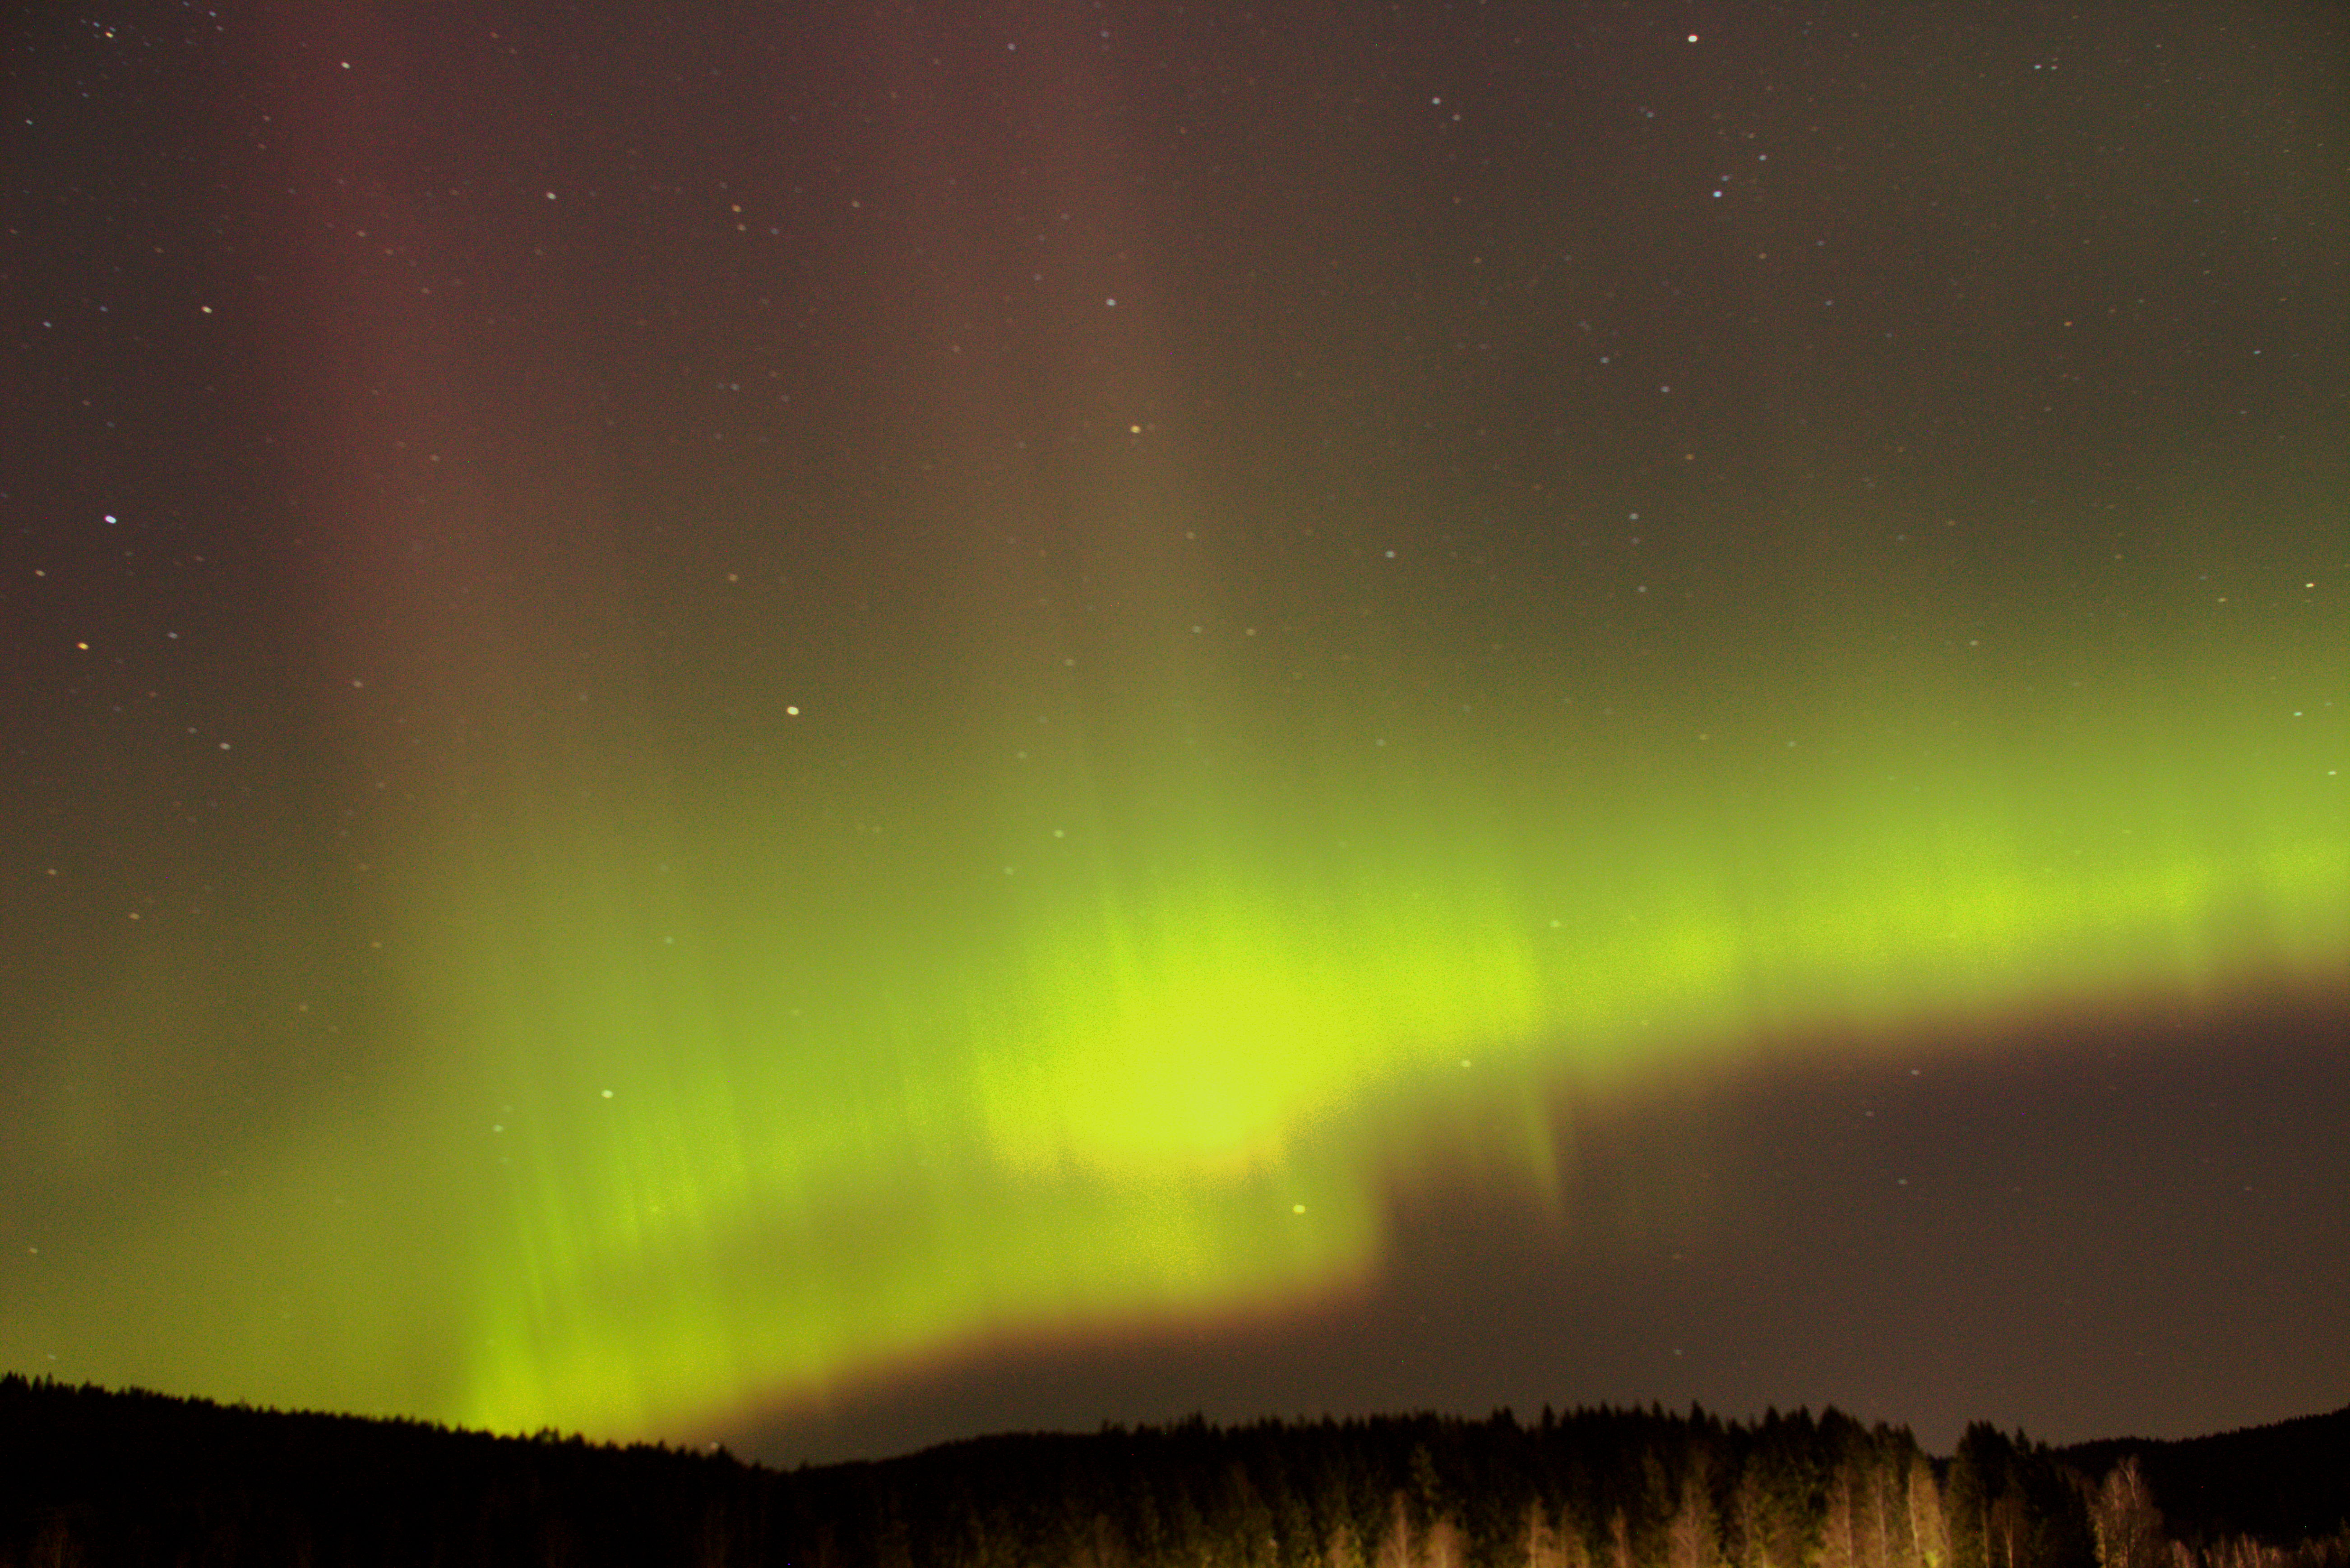
\includegraphics[width=\linewidth]{nordlys.jpg}  % inkluder et bilde. \linewidth er
	% bredden mellom margene.
	\caption{Fotografi av nordlys sett fra Sognsvann 16. Mars 2023.} % figurtekst
	\label{fig:nordlys} % så du kan henvise til figuren fra teksten.
\end{figure}

På samme måte som for overskrifter og likninger kan du henvise til figurer. \Cref{fig:nordlys}
er et .jpg bilde, men de fleste formater støttes. Når du lager en figur i f.eks. python er det
best å lagre den som pdf: da slipper du pikselering.

\section{Kode}
Det er ofte nødvendig å ta med programkode i dokumentet. Det er dette som er den viktigste funksjonen til pakken listings. Den gir deg mulighet til å bestemme akkurat hvordan koden skal
se ut. I \cref{lst:terning} kan du se et eksempel, merk at du kan referere til kode på samme
måte som til figurer, men label og caption settes som argumenter i komandoen
\lstinline$\lstinputlisting$, ikke med egne kommandoer. 
Innstillingene kan settes både i dokumentet og i preamble. Se dokumentasjonen for detaljer.

\lstinputlisting[language=python, caption={Et enkelt program for å trille terninger.},
	label={lst:terning}]{terning.py}

\end{document}
